% !TEX root = ../../../I4PRJ, Grp3 - Rapport.tex
\section{Web GUI}
Web-applikationen benytter ASP.NET MVC framework. Controllerklasserne er lavet således, at de implementerer hvert view-interface i præsentationslaget. Broen mellem ASP.NET MVC og den overordnede MVP arkitektur sker altså ved implementering af førnævnte interfaces.

Designet af Application.Web
\begin{figure}
	\centering
	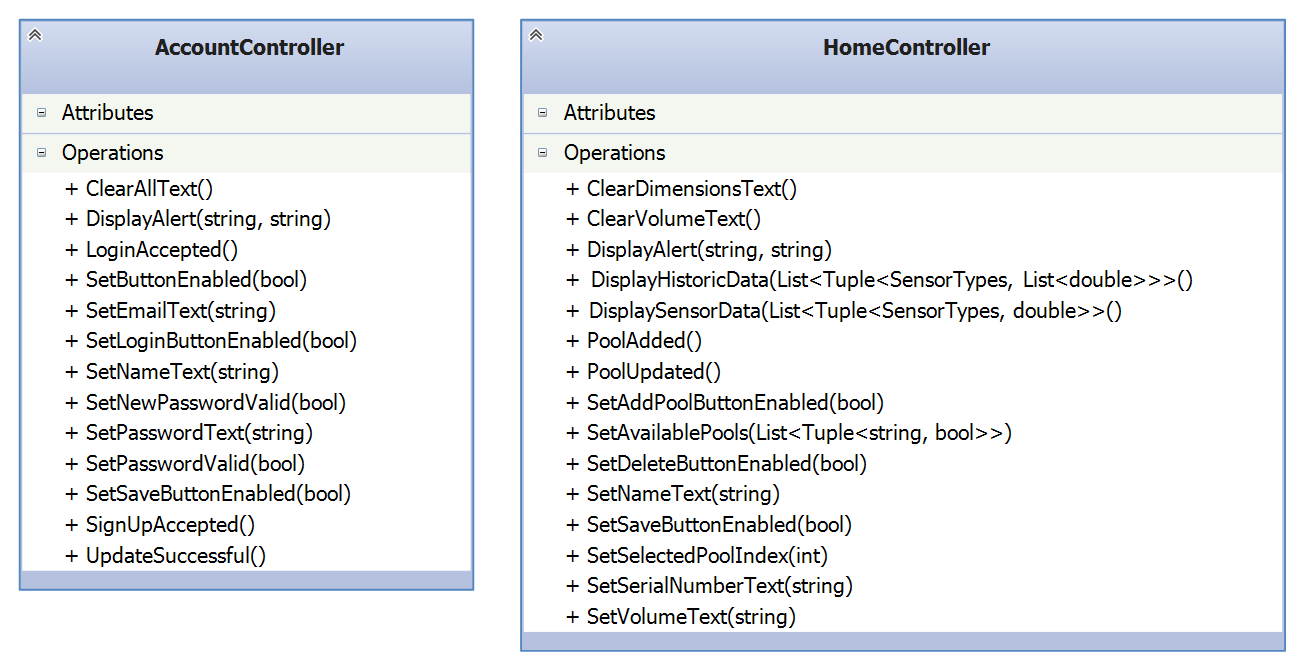
\includegraphics[width=0.9\linewidth]{figs/design/application_web}
	\caption{Web applikations design}
	\label{fig:web_class}
\end{figure}

På figur~\ref{fig:web_class} ses hvilke controllers som implementerer, hvilke interfaces. AccountController implementerer alt som har med brugeren at gøre, såsom login og signup. Homecontroller implementerer alt som har med pools og status på poolen at gøre. Designet er et indledende design og beslutningen om hvorvidt særligt Homecontroller skal have så meget ansvar er en antagelse. Det skyldes Web-applikationen begrænsede udvikling, som en iterativproces. Den iterative design- implementering- og testproces, har kun haft et fuldt gennemløb, for LoginView. 

